\chapter*[Introdução]{Introdução}
\addcontentsline{toc}{chapter}{Introdução}

Este documento é definido como um conjunto de pesquisas e descri\c{c}\~oes de atividades que ir\~ao resultar em um projeto de melhorias que utilizam exclusivamente solu\c{c}\~oes tecnol\'ogicas para o Parque Urbano do Gama-DF. Esse projeto deve ser detalhado de modo a ser poss\'ivel uma futura utiliza\c{c}\~ao das ideias aqui descritas atrav\'es de simula\c{c}\~oes, esquem\'aticos e texto descritivo. 

\section{Contextualiza\c{c}\~ao}

O Parque Vivencial do Gama localiza-se na Regi\~ao Administrativa II do Gama, criada atrav\'es da Lei n.$^o$ 49/89 e do Decreto n.$^o$ 11.921/89 e formada por \'area urbana e rural. A \'area urbana \'e dividida em seis setores, sendo: Norte, Sul, Leste, Oeste, Central e de Ind\'ustria. O Parque Vivencial do Gama est\'a localizado no setor Norte (coordenadas 16 $^o$ 00`13.4``S 48 $^o$03`55.0``W), ocupando uma \'area de aproximadamente 52 mil m$^{2}$ \cite{COEX}. A Figura abaixo apresenta a imagem da \'area do parque.

\begin{figure}[H]
	\centering
	\label{Imagem do Parque Vivencial do Gama}
		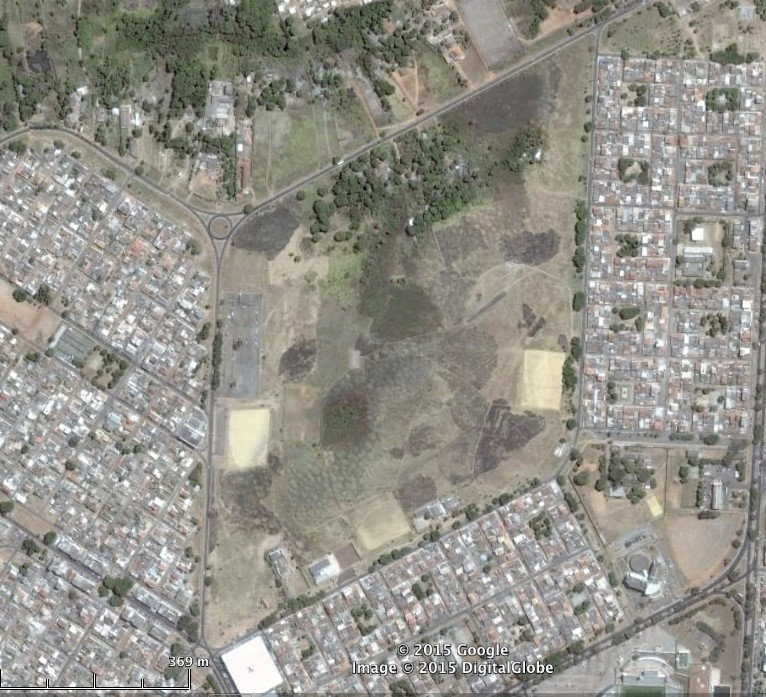
\includegraphics[keepaspectratio=true,scale=0.6]{introducao/ParqueVivencialGama.jpg}
	\caption{Imagem do Parque Vivencial do Gama}
	\small{Fonte: Google, 2015}
\end{figure}
